\chapter{Bausteinsicht}
Die Bausteinsicht ist der Grundrissplan einer jeden Software. Für die Anwendung eCourse ist die Bausteinsicht in Abbildung \ref{fib:Bausteinsicht} dargestellt.
Diese Darstellung ist eine statische Zerlegung des Systems in Bausteine. Diese Ansicht ermöglicht es vor allem die Kommunikation zwischen den Entwicklern untereinander bzw. mit dem Stakeholder zu erleichtern, da sie das System abstrahiert und dadurch von der Besprechung von Implementierungsdetails entbindet

\begin{figure}[H]
\centering
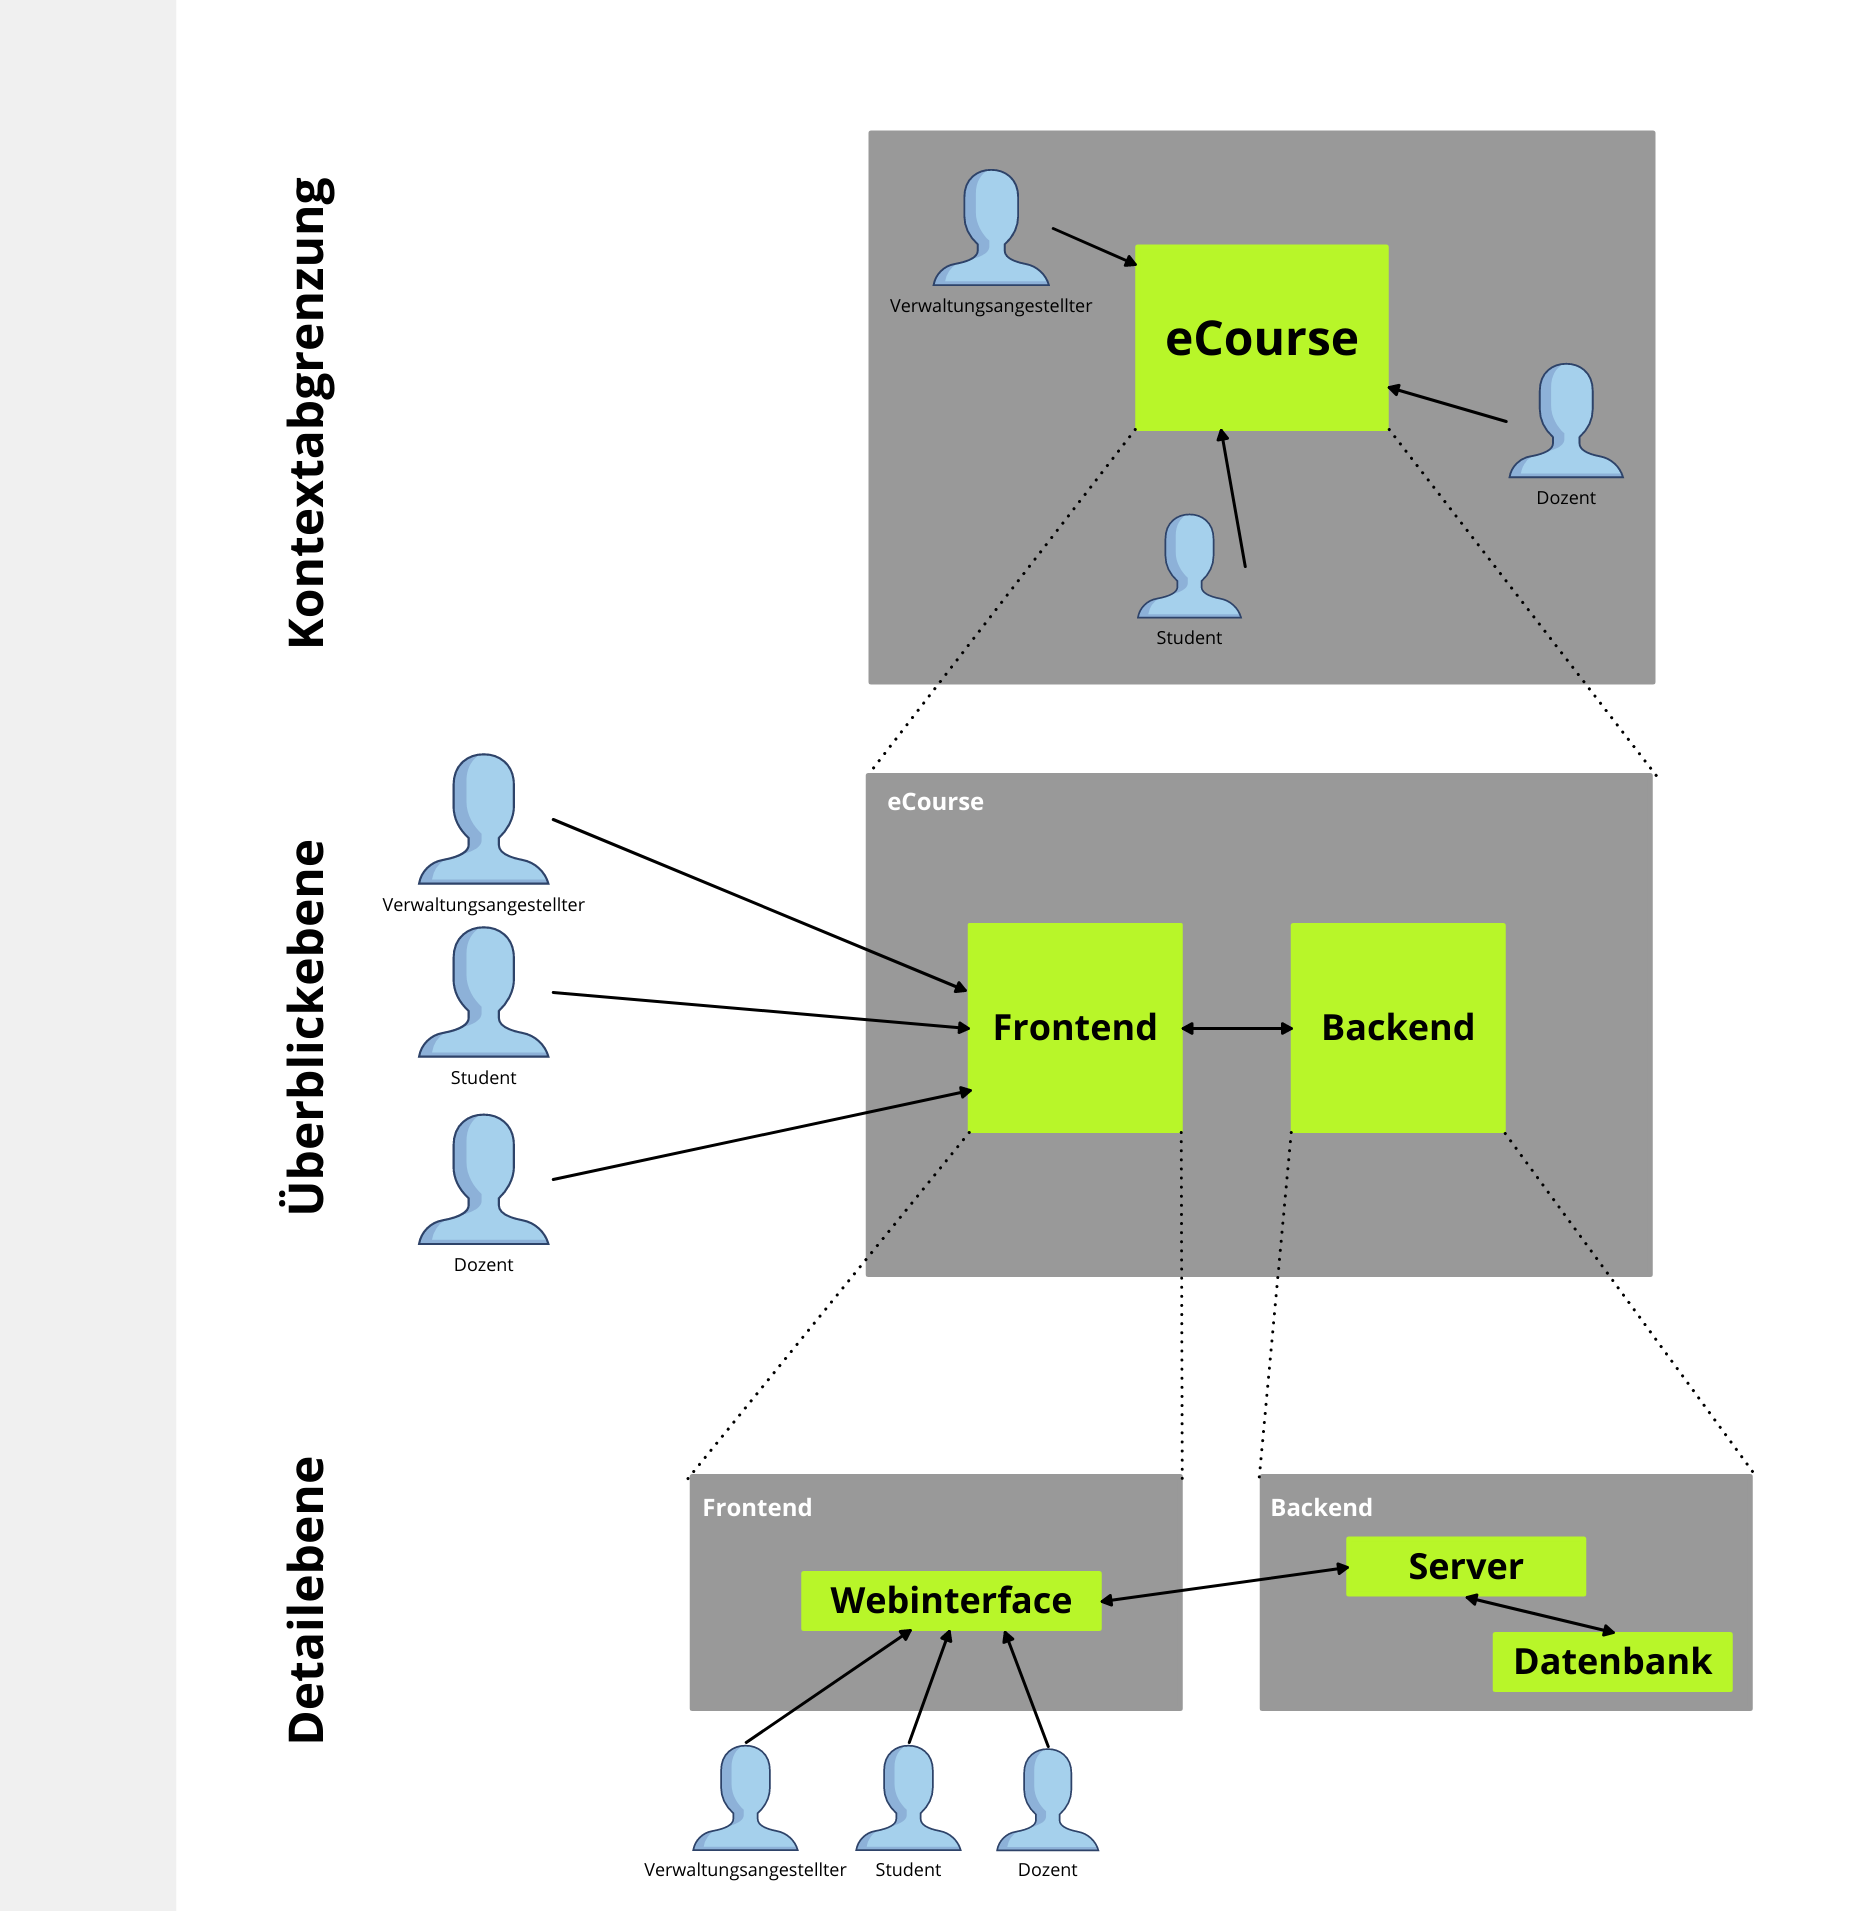
\includegraphics[height=1.0\textwidth]{Bausteinsicht.png}
\caption{Bausteinsicht für die Anwendung eCourse}
\label{fib:Bausteinsicht}
\end{figure}
